\documentclass{article}
\usepackage[papersize={20cm,12cm},margin=0.4cm]{geometry}
\usepackage{lmodern}
\usepackage{tikz}
\usetikzlibrary{arrows.meta,positioning,fit,backgrounds}
\pagestyle{empty}
\begin{document}
\centering
\vspace*{\fill}
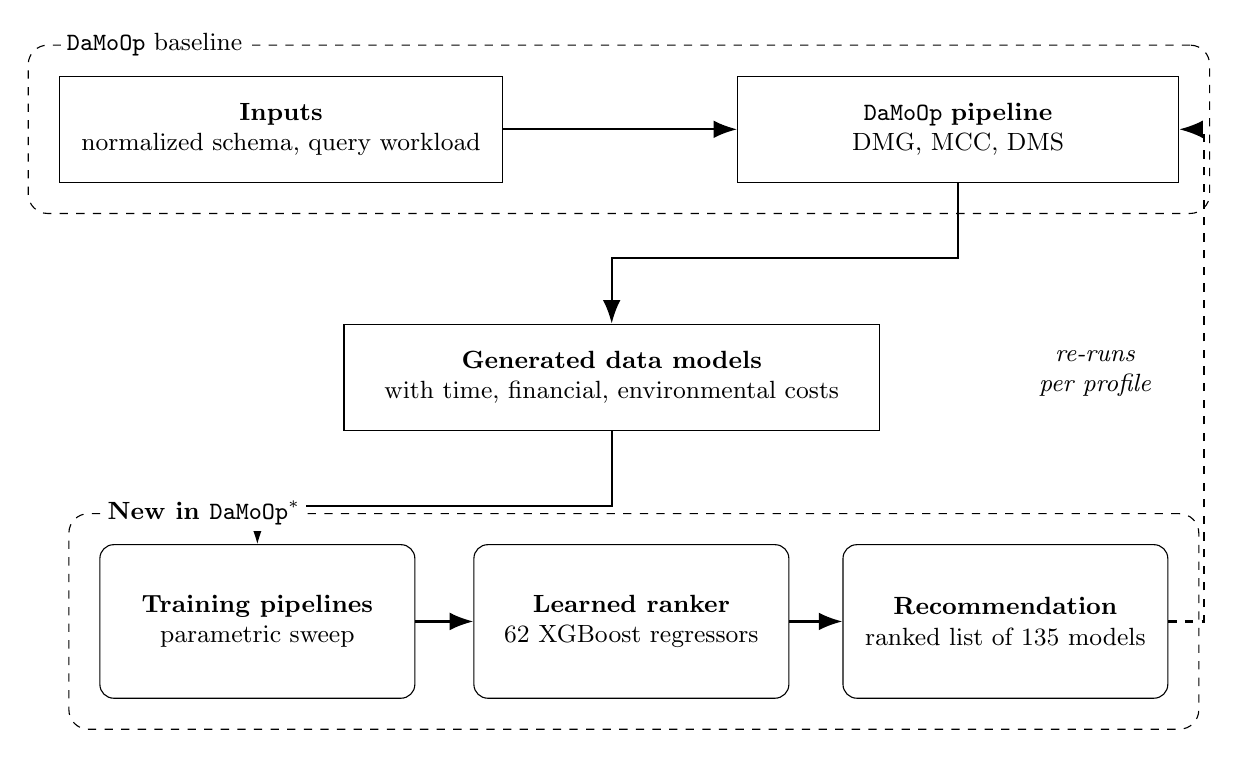
\begin{tikzpicture}[
  font=\small,
  box/.style={draw, rectangle, align=center, inner xsep=8pt, inner ysep=7pt,
              minimum height=1.35cm},
  rbox/.style={box, rounded corners=5pt, minimum height=1.95cm, minimum width=4.0cm},
  grp/.style={draw, dashed, rounded corners=7pt, inner sep=11pt},
  ar/.style={-{Latex[length=3mm]}, thick},
  dar/.style={-{Latex[length=3mm]}, thick, dashed},
]

% ---- top row: DaMoOp baseline ----
\node[box, minimum width=5.6cm] (inp) at (3.5,7.9)
  {\textbf{Inputs}\\ normalized schema, query workload};
\node[box, minimum width=5.6cm] (pipe) at (12.1,7.9)
  {\texttt{DaMoOp} \textbf{pipeline}\\ DMG, MCC, DMS};
\draw[ar] (inp) -- (pipe);

% ---- middle: generated data models ----
\node[box, minimum width=6.8cm] (gen) at (7.7,4.75)
  {\textbf{Generated data models}\\ with time, financial, environmental costs};
\draw[ar] (pipe.south) -- ++(0,-0.95) -| (gen.north);

% ---- bottom row: New in DaMoOp* ----
\node[rbox] (train) at (3.2,1.65) {\textbf{Training pipelines}\\ parametric sweep};
\node[rbox] (rank)  at (7.95,1.65) {\textbf{Learned ranker}\\ 62 XGBoost regressors};
\node[rbox] (rec)   at (12.7,1.65) {\textbf{Recommendation}\\ ranked list of 135 models};
\draw[ar] (train) -- (rank);
\draw[ar] (rank) -- (rec);

% data flow: generated -> training (elbow down-left)
\draw[ar] (gen.south) -- ++(0,-0.95) -| (train.north);

% re-run loop (dashed) up the right side back into the pipeline
\draw[dar] (rec.east) -- ++(0.45,0) |- (pipe.east);
\node[align=center] at (13.85,4.8) {\textit{re-runs}\\ \textit{per profile}};

% ---- dashed group frames ----
\begin{scope}[on background layer]
  \node[grp, fit=(inp)(pipe)] (bg1) {};
  \node[grp, fit=(train)(rank)(rec)] (bg2) {};
\end{scope}
\node[fill=white, inner sep=2pt, anchor=west] at ([xshift=12pt]bg1.north west)
  {\texttt{DaMoOp} baseline};
\node[fill=white, inner sep=2pt, anchor=west] at ([xshift=12pt]bg2.north west)
  {\textbf{New in \texttt{DaMoOp}$^{*}$}};

\end{tikzpicture}
\vspace*{\fill}
\end{document}
